%%%%%%%%%%%%%%%%%%%%%%%%%%%%%%%%%%%%%%%%%%%%%%%%%%%%%%%%%%%%%%%%%%%%%%%%%%%%%%%
% Chapter 4 : Título del Capítulo cuatro
%%%%%%%%%%%%%%%%%%%%%%%%%%%%%%%%%%%%%%%%%%%%%%%%%%%%%%%%%%%%%%%%%%%%%%%%%%%%%%%

La plataforma desarrollada para el Trabajo Fin de Grado, llamada ``CodeCharts'', está destinada a mostrar los resultados de alumnos que han realizado cursos o talleres de Pensamiento Computacional, de manera gráfica.
Permite al profesorado crear cursos e insertar todos los datos referentes a sus alumnos en ellos.

\begin{figure}[!th]
\begin{center}
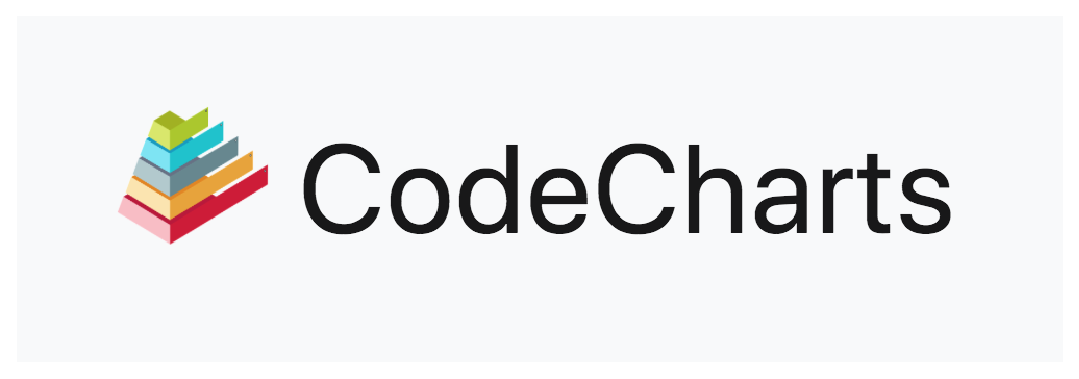
\includegraphics[width=0.5\textwidth]{images/logo_plataforma.eps}
\label{fig:9}
\end{center}
\end{figure}

En las siguientes secciones se describen en detalle la arquitectura y el diseño de la aplicación.

%++++++++++++++++++++++++++++++++++++++++++++++++++++++++++++++++++++++++++++++

\section{Arquitectura de la aplicación}
\label{4:sec:1}

\subsection{CodeCharts}
\label{1:sec:1}

CodeCharts fue desarrollado en Ruby on Rails, como se menciona en el punto 3.3.1, siguiendo la estructura en este tipo de proyectos ``MVC'' (Modelo, Vista, Controlador), así como el resto de herramientas que se describen en dicho capítulo.

%++++++++++++++++++++++++++++++++++++++++++++++++++++++++++++++++++++++++++++++

\newpage
\subsection{Base de datos}
\label{1:sec:2}

Desde un principio se usó una base de datos relacional, que nos proporcionaba Rails a través de SQLite y ActiveRecord.

\begin{figure}[!th]
\begin{center}
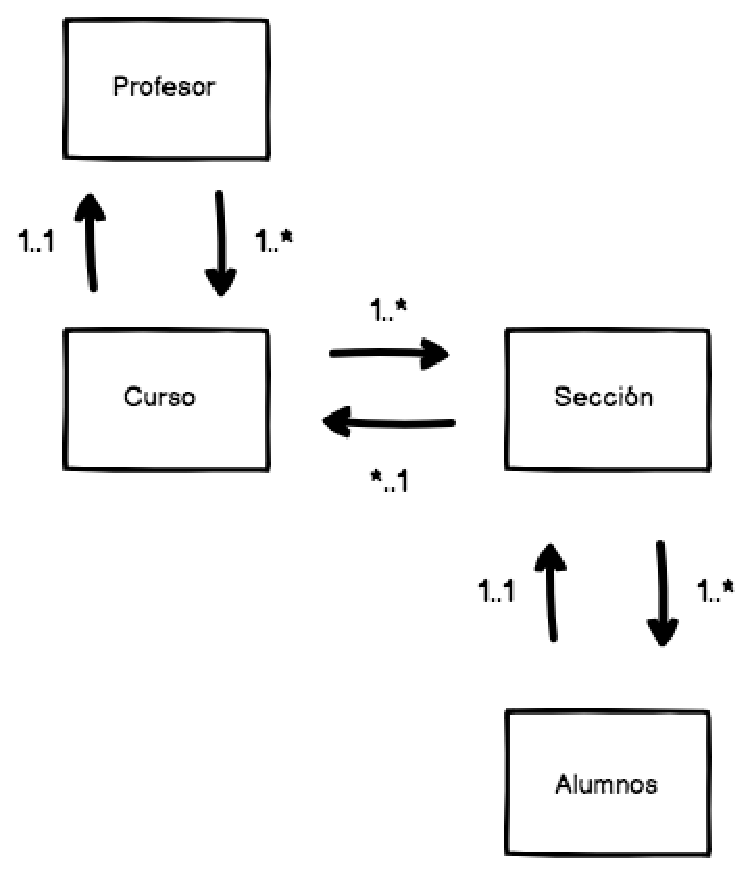
\includegraphics[width=0.4\textwidth]{images/base_de_datos.eps}
\caption{Esquema de la Base de Datos}
\label{fig:10}
\end{center}
\end{figure}

Como se muestra en la figura~\ref{fig:10}, la estructura de la base de datos se divide en cuatro tablas:

\begin{itemize}
    \item Profesor: donde se almacena toda la información referente a los profesores que se registren en la plataforma.
    \item Curso: creados por el profesorado, se guarda la información detallada del curso (título, descripción, etc.).
    \item Sección: se podría definir como el lugar de realización del curso, como por ejemplo ``Arona'', que tiene registrados a los alumnos con sus resultados en el mismo.
    \item Alumno: tabla en la que se almacenan los datos, así como los resultados, de los estudiantes que realizan los cursos o talleres de pensamiento computacional.
\end{itemize}

%++++++++++++++++++++++++++++++++++++++++++++++++++++++++++++++++++++++++++++++

\subsection{Gemas utilizadas}
\label{1:sec:2}

Una de las funcionalidades y características que tiene Ruby, el lenguaje usado para desarrollar el proyecto, es la incorporación de gemas, al igual que ocurre con el entorno NodeJS y sus paquetes ``npm''.

CodeCharts posee algunas relevantes como:

\begin{itemize}
    \item \textbf{Rails}, la gema que incluye Ruby on Rails por defecto para la utilización del framework.
    \item \textbf{SQLite}~\cite{SQLite}, para el manejo de las bases de datos, así como ActiveRecord.
    \item \textbf{Devise}~\cite{Devise}, que ofrece una solución flexible para la autenticación de los usuarios en la aplicación.
    \item \textbf{Bootstrap}~\cite{BootstrapGem}, gema que permite el diseño del front-end de la plataforma con Bootstrap.
    \item \textbf{Will-paginate}~\cite{Paginate}, de manera que si hay una gran cantidad de usuarios dentro de una sección, permita agruparlos en páginas.
    \item \textbf{Wicked-pdf}~\cite{WickedPDF}, con lo que el profesor puede descargar en formato .PDF los resultados de los alumnos.
    \item \textbf{Chartkick}, herramienta que muestra en forma gráfica los resultados obtenidos en los test de los estudiantes.
    \item \textbf{Jquery-rails}~\cite{JqueryRails}, que incluye Jquery en la aplicación. 
\end{itemize}

%++++++++++++++++++++++++++++++++++++++++++++++++++++++++++++++++++++++++++++++

\section{Diseño de la aplicación}
\label{1:sec:2}

\subsection{Página de inicio}
\label{1:sec:1}

La primera vez que se accede a la aplicación, el profesor, que será el usuario a registrarse en la plataforma, verá una descripción de en qué consiste la aplicación y lo que ofrece al profesorado en los cursos impartidos.

\begin{figure}[!th]
\begin{center}
\includegraphics[width=0.5\textwidth]{images/captura_inicio.eps}
\label{fig:11}
\end{center}
\end{figure}

Dentro de está página, el profesor se podrá registrar por primera vez, o por el contrario, si ya dispone de una cuenta creada previamente, puede entrar con la misma.

%++++++++++++++++++++++++++++++++++++++++++++++++++++++++++++++++++++++++++++++

\subsection{Registro/Inicio de sesión}
\label{1:sec:2}

En las capturas que se observan a continuación, el profesor puede tanto crearse una cuenta, como iniciar con una ya creada, si ya se ha registrado previamente. 
\begin{figure}[!th]%
    \centering
    \subfloat{{\includegraphics[width=5cm]{images/registro.eps} }}%
    \qquad
    \subfloat{{\includegraphics[width=5cm]{images/inicio_sesion.eps} }}%
    \caption{Registro e inicio de sesión}%
    \label{fig:12}%
\end{figure}

El formulario de \textit{creación de usuario} para la plataforma es muy sencillo, dado que consta de los datos básicos que se solicitan en la gran mayoría de páginas, como su nombre y apellidos, su correo electrónico y una contraseña.

%++++++++++++++++++++++++++++++++++++++++++++++++++++++++++++++++++++++++++++++

\subsection{Cursos creados}
\label{1:sec:3}

Una vez que el profesor ha accedido a la plataforma por primera vez, se mostrará una página como la que se observa en la figura. En ella se puede observar que se le informa al usuario que no tiene creado ningún curso/taller para sus alumnos, 
con lo que puede crearlos a través del botón de la parte superior izquierda.

\newpage
\begin{figure}[!th]
\begin{center}
\includegraphics[width=0.5\textwidth]{images/captura_cursos.eps}
\label{fig:13}
\end{center}
\end{figure}

Los cursos creados se irán mostrando al profesor en forma de cuadrícula, de manera que el tutor sepa los cursos que tiene creados, con su información asociada (título, descripción y fecha de creación).

\begin{figure}[!th]
\begin{center}
\includegraphics[width=0.5\textwidth]{images/cursos_creados.eps}
\label{fig:14}
\end{center}
\end{figure}

%++++++++++++++++++++++++++++++++++++++++++++++++++++++++++++++++++++++++++++++

\subsection{Perfil del profesor}
\label{1:sec:4}

Al profesor que haya iniciado sesión en ese momento, se le permitirá la opción de editar su perfil, a la vez que borrar su cuenta en caso de que ya no vaya a usar su cuenta en la plataforma.
Para que cualquier cambio, como se informa en el formulario, es necesaria la contraseña actual.

\begin{figure}[!th]
\begin{center}
\includegraphics[width=0.4\textwidth]{images/editar_perfil.eps}
\label{fig:15}
\end{center}
\end{figure}

%++++++++++++++++++++++++++++++++++++++++++++++++++++++++++++++++++++++++++++++

\subsection{Detalles del curso}
\label{1:sec:5}

En el momento que el docente cree el curso o taller, podrá acceder para observar los detalles del mismo, así como crear secciones dentro de la actividad.

\begin{figure}[!th]
\begin{center}
\includegraphics[width=0.5\textwidth]{images/detalles_curso.eps}
\label{fig:16}
\end{center}
\end{figure}

Al igual que con la página de las actividades, se le comunica al profesor que para observar las estadísticas de ese curso, tiene que añadir el lugar (Sección) donde se celebró el taller.
Uno de los detalles a destacar en el curso sería el de ``Valor de referencia", que se podría definir como un número representativo que indica el nivel que tienen los alumnos de media que realizan
esa actividad.

\begin{figure}[!th]
\begin{center}
\includegraphics[width=0.5\textwidth]{images/curso_secciones.eps}
\label{fig:17}
\end{center}
\end{figure}

En la captura anterior se puede observar un curso creado de ejemplo, junto con las secciones donde se realizó el curso. Tiene tanto la posibilidad de administrar a los alumnos, como se muestra en el botón derecha, al igual que eliminarlo.

%++++++++++++++++++++++++++++++++++++++++++++++++++++++++++++++++++++++++++++++

\newpage
\subsection{Detalles de la sección}
\label{1:sec:6}

El objetivo final de la plataforma es que el profesor, cuando inserte los resultados de los alumnos obtenidos de la plataforma Code.org, observe con gráficos las calificaciones de cada uno.

\begin{figure}[!th]
\begin{center}
\includegraphics[width=0.7\textwidth]{images/lista_sin_alumnos.eps}
\label{fig:18}
\end{center}
\end{figure}

\begin{figure}[!th]
\begin{center}
\includegraphics[width=0.3\textwidth]{images/insertar_alumnos.eps}
\label{fig:19}
\end{center}
\end{figure}

Se pueden registrar alumnos en la plataforma tanto de manera manual (de uno en uno), como a través de un fichero .json con la información requerida, entre la que se encuentra el nombre, apellidos, edad, etc. Entre los datos más relevantes,
los niveles completados en ese reto, así como las líneas de código utilizadas en total.

\begin{figure}[!th]
\begin{center}
\includegraphics[width=0.7\textwidth]{images/subir_fichero.eps}
\label{fig:20}
\end{center}
\end{figure}

\newpage
Al finalizar los retos por parte de los alumnos, el profesor obtendrá una tabla con toda la información de cada uno paginados, de manera que la tabla no se vuelva muy extensa al matricular a muchos alumnos, como se muestra a continuación.

\begin{figure}[!th]
\begin{center}
\includegraphics[width=0.7\textwidth]{images/tabla_alumnos.eps}
\label{fig:21}
\end{center}
\end{figure}

Por otro lado, en el apartado de estadísticas, se mostrarán gráficos desarrollados con la intención de ver en qué nivel se fomenta el aprendizaje en los alumnos.

\begin{figure}[!th]
\begin{center}
\includegraphics[width=0.7\textwidth]{images/estadisticas_seccion.eps}
\label{fig:22}
\end{center}
\end{figure}

En la imagen anterior se pueden observar algunos de los resultados obtenidos en forma de gráficos por los alumnos en ese curso.